% ****************** Introdução *********************

\chapter[Introdução]{Introdução}
O capítulo compreende a contextualização, na qual se procura ambientar o leitor nos tópicos chave do trabalho sendo, principalmente: Engenharia de Requisitos e Projetos Ágeis. A questão de pesquisa, a qual norteará essa pesquisa bem como se pretende responder ao final desse trabalho com maior propriedade e clareza, também é tratada nesse capítulo. Seguem ainda: justificativas, visando  acordar as principais contibuições do trabalho; e objetivos geral e específicos, aderentes à proposta, e já direcionando o leitor para os resutados esperados com a realização desse trabalho. Por fim, tem-se a organização desse monografia, distribuída em capítulos. 

\section{Contextualização}
De acordo com \cite{tabassam2019comparative}, qualquer abordagem pode ser usada com qualquer técnica de modelagem, e isso é puramente decidido por engenheiros de requisitos com a ajuda de várias restrições, tais como: tipo de projeto, seu domínio, escopo, ambiente de negócios, usuários finais-alvo e partes interessadas que agregam como fatores decisivos da técnica de modelagem e abordagem de Engenharia de Requisítos a ser usada para aquela técnica de modelagem selecionada.

Considerando especificamente o escopo das  \textit{startups} de software, tem-se que a elicitação de requisitos 
é particularmente desafiadora nesse contexto, com base nos estudos realizados pelos autores \cite{rafiq2017requirements}. Os autores relatam que esse desafio é intensificado, uma vez que as \textit{startups} buscam por projetos de alta incerteza, os quais são vistos como oportunidades de negócio únicas, bem como de aplicação de tecnologias de ponta. Sendo assim, o domínio, na maioria das vezes, é pouco ou nada conhecido. Esse nicho de empresas ainda carece de outras iniciativas, capazes de mitigar as incertezas. Uma carência evidenciada pelos autores  \cite{rafiq2017requirements} é a falta de estudos que investigam como aproximar a camada de Requisitos de Software e a necessidade de desenvolvimento ágil, coerente com entregas rápidas e em atendimento às demandas de mercado.

Com base em \cite{lampa2017project}, tem-se que a falta de compreensão dos requisitos de um projeto é outro fator que dificulta a realização das atividades compreendidas na Engenharia de Requisitos, pois por vezes os \textit{stakeholders} não possuem pleno conhecimento de suas necessidades no início do projeto. Assim, mudanças de escopo são comuns ao longo do ciclo de vida do projeto, aumentando os esforços, os custos e os prazos. 

Diante do exposto, na sociedade comercial moderna, à medida que a tecnologia da informação se desenvolve bem como dados os variados tipos de negócios e as constantes mudanças ambientais, alinhar os requisitos torna-se cada vez mais intangível, trazendo desafios à Engenharia de Requisitos tradicional \cite{jun2010application}.

Considerando as dificuldades encontradas na Engenharia de Requisitos tradicional, surge uma nova abordagem, a Engenharia de Requisitos Ágil \cite{jun2010application}. Essa procura alterar o status atual da Engenharia de Requisitos Tradicional, buscando conformidade com as constantes mudanças dos requisitos ao longo do ciclo de vida do software.Trata-se de uma proposta de inovação em relação aos métodos tradicionais, sendo a abordagem ágil composta por um conjunto otimizado de práticas ágeis \cite{jun2010application}. 

Enquanto a aplicação de princípios ágeis leva a um melhor sucesso do projeto, alguns projetos ainda falham devido à compreensão insuficiente dos requisitos exatos do cliente. Dessa forma equipes ágeis começaram recentemente a adotar as práticas do \textit{Design Thinking} para entender melhor o que está na mente dos clientes \cite{prasad2018adopting}.

Com o intuito de revolucionar os métodos e práticas ágeis, a Google Ventures (GV) parte da Google focada em testar e acelerar ideias que ainda estão em estágio inicial de desenvolvimento. lança o método Design Sprint, baseado no processo de design 'express'. Um processo formado por um grupo de pessoas especialista nas áreas de interesse, que se reunem durante cinco dias para alinhar, levantar, definir, prototipar e testar ideias, permitindo assim que não seja necessário lançar um MVP para descobrir se a ideia é boa ou não, processo esse que pode tomar vários meses, o  \textit{Design Sprint} foca especificamente na validação da ideia com usuários e encurta o processo para 40 horas de trabalho, conforme explicado por \cite{knapp2016sprint}. Logo, o uso deste método auxilia quanto a caputura de conceitos utilizados no mesmo para o desenvolvimento de uma nova abordagem, desta vez focada em novo cenário: Elicitação, Modelagem e Análise de requisítos, originando o método \textit{Requirements Sprint}.

\section{Questão de Pesquisa}
Tendo como objetivo guiar o trabalho, foi definida a seguinte questão de pesquisa:
De que maneira a implementação conjunta de conceitos provenientes das práticas ágeis e do método Design Sprint podem contribuir para o desenvolvimento de uma abordagem capaz de apoiar a fase inicial de elicitação, modelagem e análise de requisitos em empresas e/ou organizações de pequeno ou médio porte.

\section{Justificativa}

Ao longo das décadas, a importância da elicitação de requisitos tem sido amplamente reconhecida. De fato, essa fase inicial do processo de engenharia de requisitos é crucial para reunir as informações e os dados necessários para especificar os requisitos relevantes. Os erros nessa fase podem ser transferidos nas fases subsequentes do desenvolvimento do software e comprometer o processo geral ou aumentar o custo do desenvolvimento \cite{spoletini2017requirements}.

A rápida mudança no campo da engenharia de software, em particular o surgimento de metodologias de desenvolvimento de software, diminuiu a necessidade de uma definição bem definida dos requisitos. Uma característica primária do processo no desenvolvimento de um sistema com requisitos mal definidos é a iteração através de uma ou mais fases de desenvolvimento antes que os requisitos sejam esclarecidos \cite{requirementsanalysis}

Com a finalidade de secundar a questão de pesquisa, foi proposto o desenvolvimento de uma abordagem de elicitação, modelagem e análise de requisítos baseada no método Design Sprint, desenvolvido pela Google Ventures (GV) no qual fundamenta-se em estabelecer os requisítos do sistema por meio da dedicação de uma sprint(cinco dias), para apoiar e agilizar o processo de desenvolvimento de empresas ou startups em estágio inicial por meio da integração de práticas ágeis ao processo.
\newpage
\begin{figure}[h]
\centering
\label{fig01}
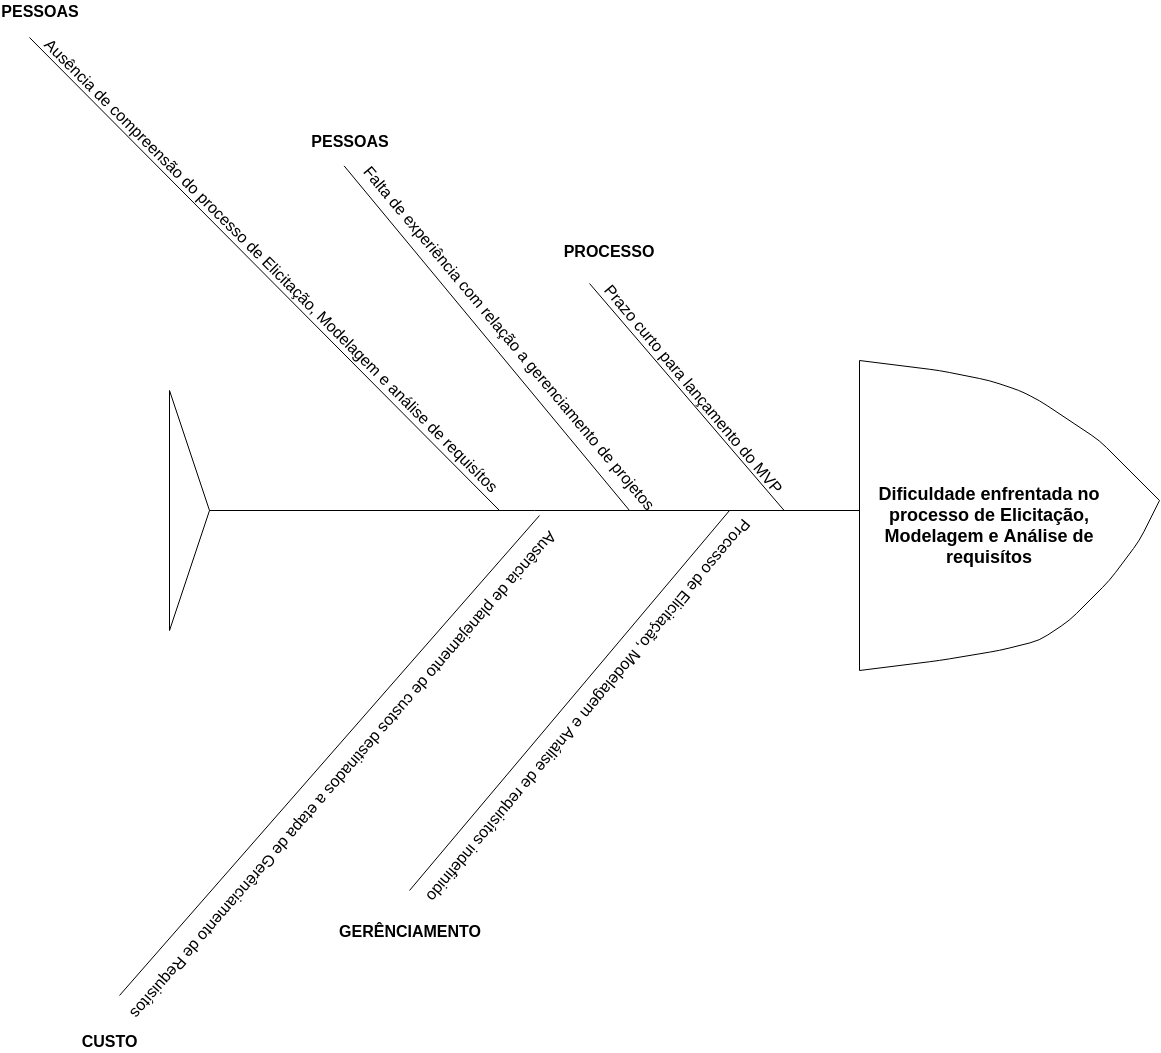
\includegraphics[keepaspectratio=true,scale=0.4]{figuras/Untitled_Diagram.png}
\caption{Diagrama de causa e efeito (fishbone).}
{Fonte: Autor}
\end{figure}
\newpage
\subsection{Revisão Sistemática}

Com objetívo de reunir materiais semelhantes de autores citados, interpretar dados,expandir conhecimentos a serem abordados no referêncial teórico e orientar investigações futuras, foi realizado a construção de um estudo secundário baseado nas fases da revisão sistemática definidas por \cite{kitchenham2004procedures}, \cite{brereton2007lessons} e a técnica "Snow Ball" no qual pode ser analisado no Apêndice \hyperlink{A}{A}.

\section{Objetivo Geral}
Elaborar uma abordagem, que auxilie organizações, empresas ou startups em estágio inicial que possuem projetos internos e/ou ideias que precisam ser amadurecidas com relação a fase de elicitação, modelagem e análise de requisítos, a fim de tornar esse processo mais simples, rápido e eficiente por meio da aplicação da mesma no ciclo de vida do processo.

\subsection{Objetivos Específicos}
Para realização deste trabalho foram considerados 
os seguintes objetivos específicos:

1. Definir por meio de revisão bibliográfica, aspectos da metodologia Design Sprint a serem utilizadas no desenvolvimento da abordagem;


2. Definir por meio de revisão bibliográfica, aspectos do Ágil a serem utilizados no
desenvolvimento da abordagem;

3. Definir um conjunto de atividades, por meio da implementação da abordagem Requirements Sprint que em conjunto com as práticas ágeis será caracterizada como a abordagem proposta;

4. Aplicar a abordagem desenvolvida em uma organização que possui as caracteristicas definidas anteriormente para aplicação do processo.

5. Avaliar resultados coletados a partir da aplicação do processo resultante da abordagem.

\newpage
\section{Organização do Trabalho}
Este documento está dividido em capítulos, sendo eles:

\textbf{Capítulo 2 - Referencial Teórico:}
 Apresenta as áreas e os conceitos relacionados ao 
 tema trabalhado.;

\textbf{Capítulo 3 - Referencial Tecnológico: }
Caracteriza as
ferramentas, frameworks e outros suportes utilizados.;

\textbf{Capítulo 4 - Metodologia: }
Especifica as escolhas
metodológicas, as atividades e o cronograma.;

\textbf{Capítulo 5 - Abordagem preliminar: }
Apresenta
a estrutura das atividades e a abordagem preliminar; 

\textbf{Capítulo 6 - Estudo de Caso: }
Apresenta a execução e análise das tarefas realizadas por meio da aplicação do processo assim 
como a concepção da
modelagem organizacional realizada por meio 
de um estudo de caso.

\textbf{Capítulo 7 - Considerações finais: }
Apresenta
os resultados alcançados, bem como possibilidade de trabalhos futuros.

% ************** Referencial Teórico *******************

\chapter[Referêncial Teórico]{Referêncial Teórico}

\section{Considerações Iniciais}
Dado o desenvolvimento da abordagem que atua em dois escopos: Engenharia de Requisitos e Projetos Ágeis, neste capítulo, será apresentado um pouco dos dois mundos. Para isso faz se necessário sintetizar os conceitos utilizados, com finalidade de elaborar um overview do que será aplicado em questão de pesquisa. Com este propósito apresentam-se a terminologia e conceitos básicos relacionados, a fim de simplificar a compreensão dos prevalecentes tópicos abordados: Engenharia de Requisítos, bem como a definição das fases de elicitação, análise E modelagem do mesmo modo que  Práticas ágeis aplicadas no contexto de projetos de pequeno e médio porte e utilização de conceitos relacionados ao método de Design Sprint.


\newpage
Dessa forma, foi desenhado um diagrama de processo de leitura de acordo com o estado atual do projeto em questão.
\begin{figure}[!htb]
\centering
\label{fig01}
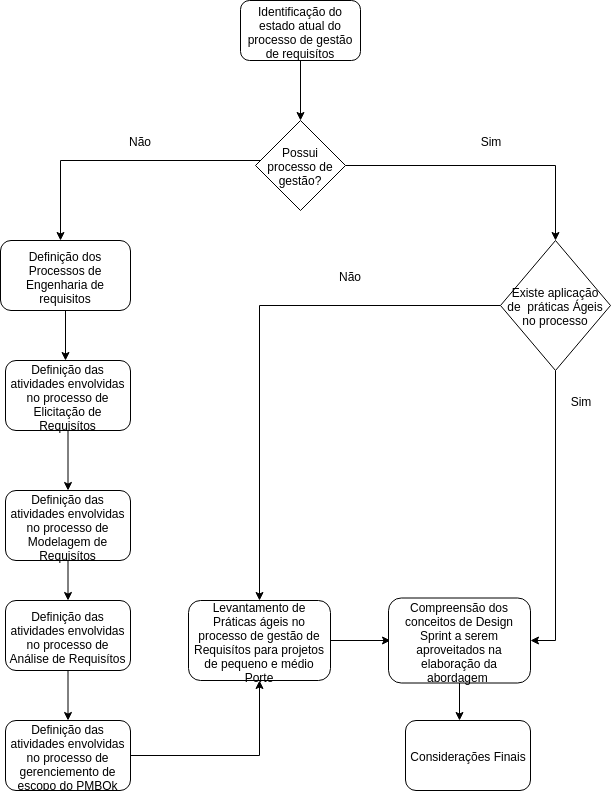
\includegraphics[keepaspectratio=true,scale=0.6]{figuras/Diagrama_de_Processos.png}
\caption{Diagrama de Processo de leitura.}
{Fonte: Autor}
\end{figure}
\newpage

\section{Engenharia de Requisítos}
De acordo com \cite{sommerville1997requirements} A engenharia de requisitos é o processo de descoberta, documentação e gerenciamento dos requisitos para um sistema baseado em computador. O objetivo da engenharia de requisitos é produzir um conjunto de requisitos do sistema que, na medida do possível, seja completo, consistente, relevante e reflita o que o cliente realmente deseja. Embora esse ideal seja provavelmente inatingível, o uso de uma abordagem sistemática baseada em princípios de engenharia leva a melhores requisitos do que a abordagem informal que ainda é comumente usada. 

Conforme descrito por \cite{riaz2018customization} existem muitos factores que podem desempenhar um papel na taxa de sucesso de projetos para qualquer organização, mas técnicas de engenharia de requisitos utilizadas pela organização é o factor-chave. De acordo com um estudo, falhas durante a fase de engenharia de requisitos podem
influenciar significativamente os processos de desenvolvimento de
qualquer projeto. De acordo com \cite{riaz2018customization} os requisitos não descobertos durante
fases de engenharia de requisito podem custar 200 vezes
mais para a correção nos estágios posteriores. 
 
Os autores \cite{arias2018framework} enfatizam que informações estruturadas e organizadas podem ser exploradas com menos esforço,
para encontrar componentes reutilizáveis quando novos requisitos aparecem. A fim de apoiar este processo, a gestão de requisítos surge de acordo com \cite{cuevas2004assessment} como uma abordagem sistemática para identificar, documentar, organizar e rastrear todos os Requisitos. No qual o principal objetivo é estabelecer um acordo entre o cliente e a equipe de software sobre o significado dos requisitos. A qualidade na de gestão de Requisitos é fundamental para o sucesso do processo de software.

\subsection{Identificando estado atual do processo de gestão de requisitos}

O autor \cite{cuevas2004assessment} defende a ideia de que, embora processo de gestão de requisitos não é realizado em
muitas organizações há algumas pessoas dentro das
organizações que executam algumas práticas de gestão de requisitos. No entanto, essas práticas
geralmente não são documentadas e como consequência não são disseminadas pela organização. 

Logo, \cite{cuevas2004assessment} propõe
uma metodologia de avaliação baseada em um questionário de dois estágios para identificar quais práticas do processo de gestão de requisitos são executadas, mas não documentadas, que práticas exigem ser priorizadas e que não são implementados devido à má gestão ou desconhecimento. Dessa forma, a fim de validar a metodologia de avaliação, o questionário foi
aplicado a um estudo de caso industrial. 

De acordo com \cite{cuevas2004assessment} o questionário proposto baseou-se na práticas dos processo de gestão de requisítos estabelecido pelo
CMMI e é dividido em duas etapas:

A primeira etapa definida por \cite{cuevas2004assessment}
relaciona-se com as práticas específicas, sendo aplicada aos funcionários que
executam os processos como: analista, desenvolvedores,
designers, programadores, entre outros. Esta fase é dividida em
cinco práticas específicas apresentadas na figura [3].

Já a segunda etapa, de acordo com \cite{cuevas2004assessment} é aplicada aos funcionários
que gerenciam o processo como: Senior,
gerente de software ou líderes de equipe.
Esta etapa é dividida em dez práticas genéricas apresentadas na figura [4], e
pretende-se por meio desta identificar se o gerenciamento de requisitos está ou não institucionalizado.

A institucionalização é conceituada por \cite{cuevas2004assessment} como um aspecto crítico da
melhoria do processo e implica que o processo é
na forma como o trabalho é realizado. Nas tabelas abaixo é especificado as práticas existentes em cada etapa.

\newpage
\begin{figure}[!htb]
\centering
\label{fig01}
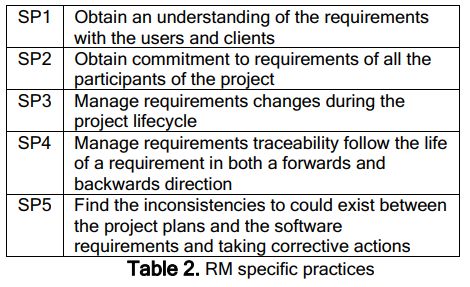
\includegraphics[keepaspectratio=true,scale=0.6]{figuras/praticas_especificas_status_projeto.png}
\caption{Praticas Específicas analisadas no formulário.}
{Fonte: \cite{cuevas2004assessment}}
\end{figure}
\begin{figure}[!htb]
\centering
\label{fig01}
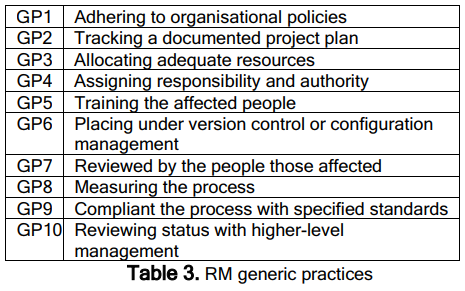
\includegraphics[keepaspectratio=true,scale=0.6]{figuras/Praticas_genericas_status_projeto.png}
\caption{Praticas Genéricas analisadas no formulário.}
{Fonte: \cite{cuevas2004assessment}}
\end{figure}
\newpage

De acordo com \cite{cuevas2004assessment} a análise dos valores obtidos a partir das
respostas dadas por meio da aplicação da primeira etapa do questionário a este caso de estudo constatou que nenhuma das cinco práticas específicas atinge o
nível de desempenho mínimo que foi definido como (75\%) para ser considerado como ponto forte no processo.
No entanto, existem três práticas SP1, SP2 e
SP3 que ficaram entre 50\% e 75\% no nível de percentual do desempenho, isto sugere que o esforço de melhoria poderia ser focado apenas para documentar o processo.

Por outro lado, os valores obtidos para
as práticas, SP4 e SP5, estavam em 50\%. Este
sugere que essas práticas devem ser priorizadas em
um plano de ação organizacional. Com base na análise dos valores obtidos a partir das
respostas dadas a partir da aplicação da segunda etapa do questionário a este caso de estudo foi constatando que nenhuma das dez práticas genéricas atinge o nível mínimo de desempenho 75\% para que seja considerado um
processo institucionalizado conforme acordado por \cite{cuevas2004assessment}. 

Porém, \cite{cuevas2004assessment} afirma que esta observação foi
esperada, uma vez que nenhuma Prática Específica foi classificada igual a 75\%.
O maior valor obtido a partir do segundo estágio
questionário foi "GP3-fornecer o adequado
recursos para executar o processo de RM ". Isto significa que
que esta Prática Geral é realizada, mas apenas algumas vezes é documentada, para este caso, o plano de ação deve ser focado para documentação da prática.
Estes resultados são exibidos nas figuras abaixo.

\newpage
\begin{figure}[!htb]
\centering
\label{fig01}
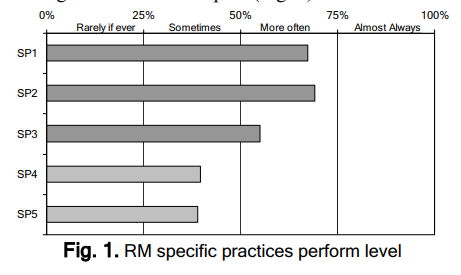
\includegraphics[keepaspectratio=true,scale=0.6]{figuras/resulto_status_praticas_especificas.png}
\caption{Resultado das Praticas Específicas aplicadas.}
{Fonte: \cite{cuevas2004assessment}}
\end{figure}
\begin{figure}[!htb]
\centering
\label{fig01}
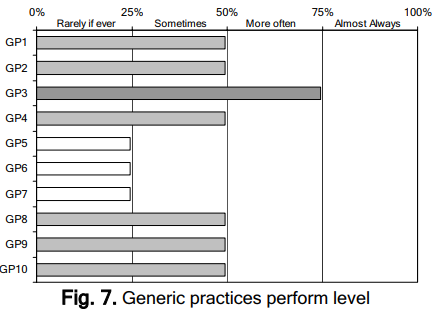
\includegraphics[keepaspectratio=true,scale=0.6]{figuras/resultados_praticas_gerais.png}
\caption{Resultado das Praticas Genéricas aplicadas.}
{Fonte: \cite{cuevas2004assessment}}
\end{figure}
\newpage

Em seguida, \cite{cuevas2004assessment} conclui que a alternativa
metodologia de avaliação baseada em duas etapas do
questionário, proposto neste artigo, poderia fornecer
informações valiosas relacionadas às áreas que exigem
Priorizar. Neste caso de estudo, duas práticas específicas
e três práticas genéricas mostraram alguns
Problemas. Estes sugerem que eles precisam ser uma prioridade
para o plano de ação.

Outra vantagem levantada por \cite{cuevas2004assessment}
metodologia baseada num questionário de duas etapas é
o auxilio na redução de custo, tempo e esforço de avaliação. Um projeto típico requer uma média
de 28 dias para o processo de avaliação e para derivar alguns resultados. No estudo de caso, o uso da
metodologia de avaliação ajudou a reduzir a avaliação
a apenas dez dias para apresentar os resultados e o plano de ação.

\cite{cuevas2004assessment} ainda afirma que a avaliação não fornece qualquer melhoria
por si só, mas fornece informações valiosas sobre a
estado atual do processo e estabelece a base para
fazer melhores escolhas sobre as mudanças que
os profissionais da tecnologia da informação devem fazer [18].
Como resultado da avaliação, deve ser gerado um plano de ação, a fim de prosseguir
projeto de melhoria. O plano de ação descreve todas as
atividades, entregáveis, cronograma e priorização de
processos a serem melhorados.

\section{Fases dos Processos de Engenharia de Requistos}

\subsection{Fase de Elicitação de Requisitos}

Conforme referido por \cite{rafiq2017requirements} a elicitação de requisitos é considerada
a primeira, principal e crucial fase dos processos de engenharia de requisitos. Inclui atividades que pretendem descobrir,
adquirir e elaborar requisitos para sistemas de software.

Para \cite{rafiq2017requirements} informações recolhidas durante a Elicitação de requisitos, muitas vezes tem de ser interpretadas, analisadas, modeladas e validadas antes para que os engenheiros se sintam confiantes de que um conjunto completo de requisitos de um sistema foram recolhidos.\cite{rafiq2017requirements} também argumentam que a seleção de técnicas de Elicitação de requisitos é dependente do problema, solução, domínio e requisitos existentes.

De acordo com \cite{rafiq2017requirements} a prática de Elicitação de requisitos depende de vários fatores,
incluindo o tipo de sistema, tipo de desenvolvimento de software e grau de adaptabilidade. Foi argumentado que a maioria das pequenas empresas são encontradas desenvolvendo sistemas que
têm requisitos orientados para o mercado. Esta característica pode também podem ser encontradas em startups de software,embora
sejam entidades diferentes do que as pequenas empresas que possui uma única missão, de escalar rapidamente apesar de seu ser tamanho pequeno inicialmente. Abaixo é apresentado um timeline referênte as técnicas de elicitação de requisítos.

\begin{figure}[!htb]
\centering
\label{fig01}
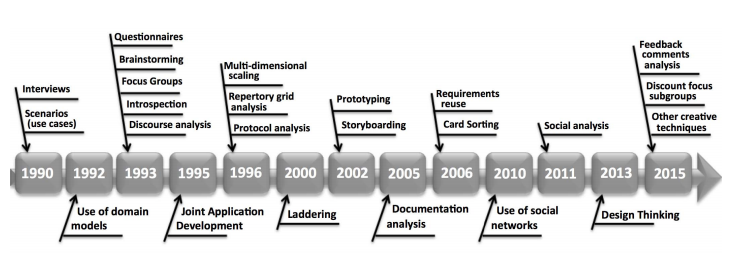
\includegraphics[keepaspectratio=true,scale=0.6]{figuras/timeline_elicitacao.png}
\caption{Timeline referênte as técnicas de elicitação de requisítos.}
{Fonte: \cite{rafiq2017requirements}}
\end{figure}

\cite{rafiq2017requirements} ainda especifica que a Elicitação de requisitos se torna mais complicada quando a natureza dos requisitos é orientada para o mercado. Requisitos tradicionais
utilizam de técnicas de Elicitação, nas quais as fontes de Elicitação são clientes ou usuários, não são apropriadas para provocar requisitos de mercado por exemplo, pois em requisitos orientados para o mercado não há clientes ou usuários específicos até que seja liberado pelo menos a versão beta para um conjunto de clientes.De forma que frequentemente requisitos orientados pelo mercado acabam sendo inventados inicialmente.

\cite{rafiq2017requirements} relata que baseado no estudo realizado nas empresas deste contexto, foi identificado que o processo de invenção é inspirado em estratégias de negócios e na visão de um produto. Mais tarde são validados e complementados com a análise de mercado. Portanto, os requisitos geralmente não são bem especificados e a linguagem natural é considerada suficiente para comunicar os requisitos e em algumas situações, os requisitos são ainda comunicados verbalmente.
As principais fontes de Elicitação de requisitos em organização de mercados de software são desenvolvedores, pessoal de vendas
e gestores. Em alguns casos, os desenvolvedores são encontrados entre os usuários pretendidos de um produto. Portanto, eles inventam requisitos baseados na sua compreensão e imaginação.

Mais tarde, quando o produto é liberado, a Elicitação é feita
examinando relatórios de bugs, feedback direto do usuário e ppor meio de técnicas serviços de apoio. No entanto, na medida em que os autores dos requisítos ficam cientes, há uma escassez dos estudos que investigam como a Elicitação de requisitos foi conduzida no específico contexto de startups de software conforme abordado por \cite{rafiq2017requirements}.

Uma abordagem de estudo de caso múltiplo realizada por \cite{rafiq2017requirements} foi empregada neste estudo
para investigar como as startups de software usam os requisitos de Elicitação ou seja as técnicas de informação, tendo em conta as informações contextuais sobre as startups. Três casos foram selecionados após uma estratégia de amostragem estratificada e prática, abrangendo diferentes tipos de aplicativos (Mobile vs. Web-based) e estágios de desenvolvimento (ideação, funcional ou maduro). São referidos como Startup 1, 2 e 3 respectivamente para a confidencialidade. Conforme apresentado na tabela abaixo.

\begin{figure}[!htb]
\centering
\label{fig01}
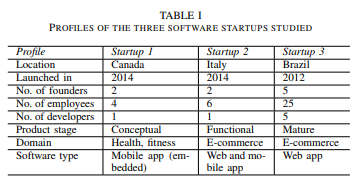
\includegraphics[keepaspectratio=true,scale=0.8]{figuras/tabela_estudo_elicitacao_startups.png}
\caption{Tabela referênte ao estudo de caso sobre técnicas de elicitação de requisítos em startups.}
{Fonte: \cite{rafiq2017requirements}}
\end{figure}

Segundo \cite{rafiq2017requirements} a maior coleta de dados foi realizada por meio de entrevistas com perguntas abertas. O projeto
das perguntas da entrevista foi guiado pelos requisitos revistos pelas
técnicas de Elicitação apresentadas na figura [7]. Para cada inicialização,o diretor de tecnologia ou o desenvolvedor sênior
foi entrevistado como o informante-chave. Cada entrevista durou
entre 60 minutos a 90 minutos. Todas as entrevistas foram
gravados e transcritos de forma textual para análise. Além disso
os sites das startups foram inspecionados cuidadosamente para obter um
melhor entendimento de suas ofertas de produtos e outras informações. Primeira análise dentro do caso e, em seguida, comparações foram realizadas. O processo de codificação foi apoiado pela utilização do
NVivo, uma ferramenta qualitativa de análise de dados.

\cite{rafiq2017requirements} descreveu o processo, especificando que antes do início do processo, os fundadores das startups já haviam
algo em mente sobre o que construir. Com o passar
do tempo, os requisitos são refinados e evoluídos praticando
um número de atividades com um foco principal na pesquisa do usuário.
A pesquisa do usuário é conduzida aplicando diversas
técnicas de Elicitação de requisitos. Este é o caso do Startup 1 e 3.
Por exemplo, a ideia inicial da Startup 3 foi um clone de
alguns negócios existentes em outro país. Mas a ideia era
ainda validada, embora informalmente, através de táticas de pesquisa do usuário antes de qualquer tipo de desenvolvimento de produto. Em vez disso, a Startup 2 não suscitava requisitos das pessoas inicialmente. A ideia inicial foi fornecida por um dos cofundadores, e os primeiros
requisitos foram inventados pela equipe.
A tabela abaixo relaciona as técnicas utilizadas nas startups estudadas.
Entre eles, entrevistas e prototipagem têm sido comumente utilizadas.

\begin{figure}[!htb]
\centering
\label{fig01}
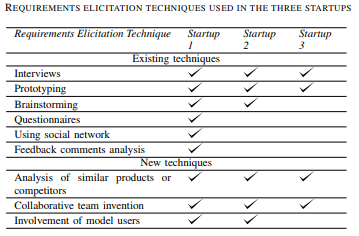
\includegraphics[keepaspectratio=true,scale=0.8]{figuras/especificacao_tecnicas_por_startup.png}
\caption{Especificação da utilização de técnicas de elicitação por startups.}
{Fonte: \cite{rafiq2017requirements}}
\end{figure}

\cite{rafiq2017requirements} destaca que três técnicas adicionais foram encontradas sendo utilizadas apenas no Startup 1, entre elas: questionários, uso de rede social e feedback por meio da análise de comentários. Estas três técnicas foram de alguma forma entrelaçadas e aplicadas em conjunto. Além de aplicar o envio de e-mail para identificar o que as pessoas precisam, fóruns de usuários relevantes e mídias sociais, também ler muitos posts,perguntas postadas e observação da reações dos usuários.

Os resultados deste estudo realizado por \cite{rafiq2017requirements} indicam que os requisitos
processo de Elicitação em startups é primordial e, principalmente, informal e é um processo contínuo ao lado da evolução do produto. A abordagem geral de Elicitação em startups é centrada numa ideia pré-concebida. Não há nenhum 
clientes identificado ou partes interessadas para extrair os requisitos diretamente. Consequentemente, as soluções concebidas baseiam-se no pressupostos e na compreensão dos fundadores do mercado.

\cite{rafiq2017requirements} menciona ainda que os achados deste estudo destacam diversas técnicas de elicitação de requisitos utilizadas em startups de software, incluindo técnicas existentes relatadas na literatura como: prototipagem, entrevistas, debate informal, questionários, utilização de redes e análise de comentários de feedback, e os novos encontrados neste estudo: análise de produtos similares ou concorrentes, discussões de equipe colaborativa e uso de usuários de modelo.

vale a pena notar segundo \cite{rafiq2017requirements} que a análise concorrente, equipe colaborativa
discussão, prototipagem e entrevistas são técnicas comuns
entre as três startups em diferentes estágios de produto.
Além disso, comparando a lista abrangente de requisitos
técnicas de Elicitação relatadas na literatura anteriormente na Figura [7] encontrados neste estudo, parece que as startups usam poucas técnicas recomendadas na literatura. Como mostrado
anteriormente, a Startup 1 (com seu produto no conceitual
(estágio) empregou todas as técnicas encontradas neste estudo
os requisitos. Em vez disso, como o produto se torna mais
concreto e maduro, menos requisitos técnicas de Elicitação
estão envolvidas, como mostrado nas startups 2 e 3. Isto pode ser tomado como indicação de que a intensidade e a frequência de utilização técnicas são diferentes durante diferentes estágios do produto.

\cite{rafiq2017requirements} conclui então que este estudo mostra que as startups não especificam ou definem requisitos explicitamente. Portanto, nenhuma documentação formal foi preparada durante ou após o processo de Elicitação de requisitos. A única documentação encontrada foi na forma de
notas, listas de tarefas e e-mails de feedback. Uma possível explicação reside na cultura Startup que é diferente da corporativa cultura em termos de orientação para o processo.

\subsection{Fase de Modelagem de Requisítos}

\subsection{Fase de Análise de Requisítos}



\section{Métodos Ágeis}

Por meio de um levantamento realizado por \cite{riaz2018customization} sobre  tipo de modelo seguido pela maioria dos
organizações o método Ágil é o mais utilizado, conforme apresentado na seguinte imagem.

\begin{figure}[!htb]
\centering
\label{fig01}
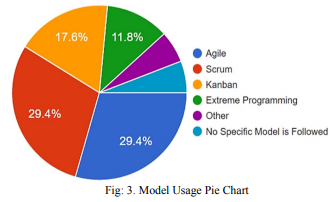
\includegraphics[keepaspectratio=true,scale=0.6]{figuras/modelo_mais_usado.png}
\caption{Levantamento de método mais utilizado para engenharia de Requisítos.}
{Fonte: \cite{riaz2018customization}}
\end{figure}

Segundo \cite{vlaanderen2011agile} uma das principais inovações no desenvolvimento de
metodologias de software dos últimos anos tem sido a introdução
de princípios ágeis. Desde a criação do manifesto ágil
em 2001, incluindo os anos que levam à sua criação,
vários métodos ágeis de desenvolvimento de software entraram em prática. Alguns exemplos são o
SCRUM, Extreme Programming e Feature
Driven Development (FDD).

Scrum é basicamente um
estrutura ágil e leve que fornece etapas para gerenciar
e controlar o processo de desenvolvimento de software e produtos.
Scrum é a combinação do modelo iterativo e o
Modelo incremental porque as compilações são sucessivas e
incremental em termos de recursos para desenvolver software orientado a objetos. Scrum foi projetado para aumentar a velocidade de
desenvolvimento, alinhar o indivíduo e as organizações,
definir uma cultura centrada no desempenho, apoiar o acionista
criação de valor, para ter uma boa comunicação de desempenho em
todos os níveis e melhorar o desenvolvimento individual e a qualidade de vida. \cite{srivastava2017scrum}

De acordo com \cite{awad2005comparison} O processo de XP pode ser
caracterizada por curtos ciclos de desenvolvimento, planejamento incremental, feedback contínuo,
confiança na comunicação, e no projeto evolutivo [9]. Com todas as qualidades acima,
os programadores respondem ao ambiente em mudança com muito mais coragem. 

Já o FDD, segundo \cite{awad2005comparison} possui um processo metodológico mais curto e que se difere do processo das demais metodologias, pois não abrange todo o desenvolvimento 
do processo de software mas centra-se nas fases de desenho e execução de funcionalidades para o projeto. Seu processo de desenvolvimento é guiado por um modelo,
uma lista de funcionalidades e o planejamento ocorre por funcionalidade, no início do projeto de forma iterativa.

Para este trabalho, o Scrum foi escolhido como a metodologia ágil base para o desenvolvimento da abordagem. A utilização de conceitos e práticas das demais metodologias abordadas não é uma impossibilidade, uma vez que cada um referidos métodos possuem práticas relevantes para contribuição com a abordagem concebida.

\subsection{Práticas Ágeis do Scrum}

Em concordância com \cite{awad2005comparison} o Scrum não requer ou fornece quaisquer métodos/práticas de desenvolvimento de software específicos
Para ser usado. Em vez disso, requer certas práticas de gerenciamento e ferramentas em diferentes fases
do Scrum para evitar o caos por imprevisibilidade e complexidade.

\cite{srivastava2017scrum} refere-se ao Scrum como um
processo que envolve um Scrum Master, o Product Owner e uma Equipe SCRUM. O principal papel do Scrum Master é eliminar impedimentos. A equipe de Scrum é uma cruz funcional que compreende de programadores, testadores e outros peritos de vários campos exigidos no desenvolvimento que conduz a um produto final versátil e inovador que atende a satisfação do cliente.

\begin{figure}[!htb]
\centering
\label{fig01}
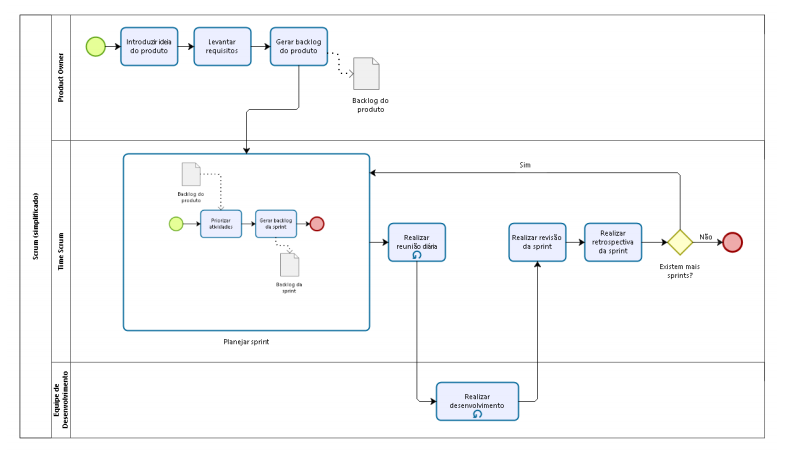
\includegraphics[keepaspectratio=true,scale=0.6]{figuras/processoScrum.png}
\caption{Processo do framework Scrum.}
{Fonte: \cite{cambraiaLeonardo}}
\end{figure}

Segundo \cite{awad2005comparison} Sprint é o procedimento de adaptação as
variáveis ambientais em mudança como: requisitos, tempo, recursos, conhecimento, tecnologia, etc) e deve resultar em um incremento potencialmente lançável de software.
As ferramentas de trabalho da equipe são: reuniões de planejamento de Sprint, Sprint backlog e Reuniões diárias do Scrum e \cite{srivastava2017scrum} especifica que uma sprint possui duração de 1 a 3
Semanas. 

Com isso algumas práticas ágeis são definidas por \cite{srivastava2017scrum} como parte do processo metodológico do Scrum, como a prática do desenvolvimento da Sprint backlog, uma documentação de todos os requisitos para Sprint atual a ser trabalhada. A Sprint Backlog é uma lista de requisitos que são determinados pelo Product Owner, resultantes do processo de engenharia de requisítos que são chamadas de histórias de usuário. Ela é seguida pela prática de planejamento de Sprint, que inclui métodos para se obter a conclusão da mesma. No final de cada dia é realizado a prática do Scrum diário
que visa o progresso da tarefa atribuída para o dia. O objectivo
da Sprint é entregar um produto potencialmente lançável.
No final de cada Sprint ocorre a prática de revisão de Sprint no qual é apresentado as atividades realizadas ao proprietário do produto para demonstrar o lançável incremento.


Segundo \cite{vlaanderen2011agile} nos últimos anos, os métodos ágeis provaram sucesso em um grande número de casos. 
Empresas que inseriram as práticas da metodologia Scrum
variam de pequenas empresas, conforme descrito por \cite{vlaanderen2011agile} para às  grandes multinacionais. 
A pesquisa demonstrou que o uso de práticas SCRUM dentro de uma empresa pode levar a benefícios significativos, e que a sua utilização não se limita a projetos locais.

\subsection{Projetos Ágeis de Pequeno e Médio Porte}

\subsection{Design Sprint - Método base para a abordagem desenvolvida}

De acordo com a Google Ventures a Design Sprint é um processo de cinco dias para responder perguntas críticas de negócios através de design, prototipagem e testar idéias com os clientes.É um "Greatest Hits" da estratégia de negócios, inovação, ciência do comportamento, Design Thinking, e muito mais-embalado em um processo de batalha testado que qualquer equipe pode usar.

Na GV as Sprints são versáteis e executadas em empresas como Nest, Flatiron Health e Medium — para ajudá-los a entrar em novos mercados, projetar novos produtos, desenvolver novos recursos para milhões de usuários, definir estratégias de marketing e muito mais. Logo, é especificado a necessidade de se definir antes de se iniciar a Sprint, o desafio e a equipe correta. Fazendo se necessário também dispor de recursos como tempo e espaço para conduzir a Sprint.O método Design Sprint é baseado em cinco dias de desenvolvimento conforme listado abaixo.

1. Segunda-Feira: As discussões estruturadas de segunda-feira criam um trajeto para a semana do Sprint. De manhã, você começará e no final concordará com um objetivo de longo prazo. Em seguida, você vai fazer um mapa do desafio. À tarde, você pedirá aos especialistas da sua empresa que compartilhem o que eles sabem. Finalmente, você escolherá um alvo: uma parte ambiciosa mas gerenciável do problema que você pode resolver em uma semana.

2. Terça-Feira: Depois de um dia cheio de compreensão do problema e escolhendo um alvo para sua Sprint, na terça-feira, você começa a se concentrar em soluções. O dia começa com inspiração: uma revisão das ideias existentes para remixagem e aperfeiçoamento. Então, à tarde, cada pessoa vai esboçar, seguindo um processo de quatro etapas que enfatiza o pensamento crítico sobre a arte. Você também começará a planejar o teste de cliente da sexta-feira recrutando clientes que se encaixam no seu perfil de destino.

3. Quarta-Feira: Na quarta-feira de manhã, você e sua equipe terão uma pilha de soluções. Isso é ótimo, mas também é um problema. Você não pode prototipar e testá-los todos — você precisa de um plano sólido. Na parte da manhã, você vai criticar cada solução, e decidir quais têm a melhor chance de alcançar o seu objetivo a longo prazo. Então, à tarde, você vai levar as cenas vencedoras de seus esboços e criar um storyboard: um plano passo-a-passo para o seu protótipo.

4. Quinta-Feira: Na quarta-feira, você e sua equipe criaram um Storyboard. Na quinta-feira, você adotará uma filosofia "falsa" para transformar esse storyboard em um protótipo. Uma fachada realista é tudo que você precisa para testar com os clientes, e aqui está a melhor parte: concentrando-se na superfície voltada para o cliente do seu produto ou serviço, você pode terminar o seu protótipo em apenas um dia. Na quinta-feira, você também vai se certificar de que tudo está pronto para o teste de sexta-feira, confirmando o cronograma, rever o protótipo, e escrever um roteiro de entrevista.


5. Sexta-Feira: Sua Sprint começou com um grande desafio, uma equipe excelente-e não muito mais. Até sexta-feira, você criou soluções promissoras, escolheu o melhor, e construiu um protótipo realista. Isso só seria possível em uma semana impressionantemente produtiva. Mas você vai dar um passo adiante, entrevistar os clientes e aprender assistindo-os reagir ao seu protótipo. Este teste faz toda a Sprint valer a pena: no final do dia, você vai saber o quão longe você tem que ir, e o que fazer e seguida.

\section{Considerações Parciais}

Acima, foi especificado o processo metodológico do Scrum, no qual para a aplicação desta abordagem, o foco neste processo se dará na etapa referente a gestão de requisitos executada pelo Product Owner da equipe, que possui a responsabilidade de levantar o planejamento conforme o problema, desenvolvendo uma Sprint Backlog sucinta as necessidades do produto e fragmenta-la para a equipe de desenvolvimento, a fim de se obter os melhores resultados com o que foi planejado na Sprint.

